\section{Algorytm Simulated Annealing}

%%%%%%%%%%%%%%%%
	
	\begin{frame}{Algorytm Simulated Annealing}
		\begin{figure}
			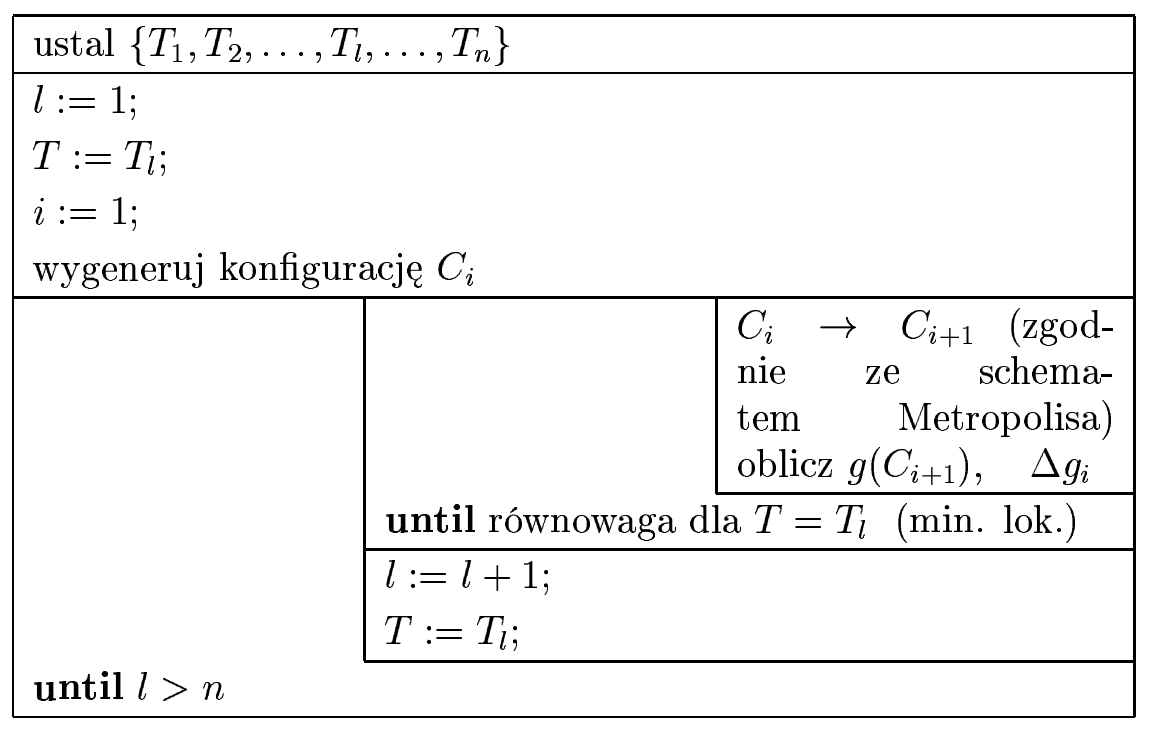
\includegraphics[width=0.8\textwidth]{img/18/sa_algorithm}
		\end{figure}
		$\{T_l\}$ - temperature schedule: $T_l > T_{l+1}$\\
		np. $T_{l+1} = 0.9 \cdot T_l$
	\end{frame}

%%%%%%%%%%%%%%%%
	\begin{frame}{Sprawdzanie, czy układ jest w równowadze}
		\begin{block}{Sposób A}
			utrzymywać $T_l$ przez $\begin{cases}
			100 \cdot N \text{ prób} \\
			10 \cdot N \text{ prób udanych} (\Delta g < 0)
			\end{cases}$
		\end{block}
		
		\begin{block}{Sposób B}
		$n$ - ustalona liczba prób ($\sim$ epoka)
		\begin{enumerate}
			\item wykonać $n$ prób ($C_i \rightarrow C_{i+1}$)
			\item zachować g(C$_n$)
			\item porównać $g_i(C_n)$ dla kilku ostatnich zestawów po $n$ próbach \\
			brak istotnej zmiany $g(C_n) \rightarrow$ nowe $T$.
		\end{enumerate}
		\end{block}
		\textbf{Start:} stopienie $\rightarrow$ 
		\begin{itemize}
			\item określić typowe $\Delta g$
			\item wybrać $T >> g$ $(\Delta E)$
		\end{itemize}
		
		
	\end{frame}
	
%%%%%%%%%%%%%%%%
	\begin{frame}{Interaktywna demonstracja działania Simulated Annealing}
		Źródła w C i C++:
		\begin{itemize}
			\item 	\url{https://www.taygeta.com/annealing/simanneal.html}
		\end{itemize}
		
		
		%Programy w C:
		%Postscript:
		% martwe linki
	\end{frame}